%==============================================================================
% AUTHBC — PhD/MSc thesis, Mohamed A. Farouk
%
% STATUS (2026-08-30). This is a DRAFT SKELETON with the technical core written.
% Chapter completeness is declared honestly in thesis/STATUS.md — do not present
% this as a finished thesis. Build:  make thesis
%==============================================================================
\documentclass[11pt,a4paper,oneside]{report}

\usepackage[T1]{fontenc}
\usepackage[utf8]{inputenc}
\usepackage{lmodern}
\usepackage[english]{babel}
\usepackage[margin=3cm]{geometry}
\usepackage{amsmath,amssymb,amsthm}
\usepackage{graphicx}
\usepackage{booktabs}
\usepackage{longtable}
\usepackage{array}
\usepackage{siunitx}
\usepackage{xcolor}
\usepackage[hidelinks]{hyperref}
\usepackage{cleveref}
\usepackage{setspace}
\usepackage{fancyhdr}
\usepackage{tikz}
\usetikzlibrary{positioning,arrows.meta,fit,backgrounds}

\graphicspath{{.}}
\onehalfspacing
\setlength{\parskip}{0.4em}

\pagestyle{fancy}
\fancyhf{}
\fancyhead[L]{\nouppercase{\leftmark}}
\fancyhead[R]{\thepage}
\renewcommand{\headrulewidth}{0.4pt}

% --- theorem environments ----------------------------------------------------
\theoremstyle{plain}
\newtheorem{theorem}{Theorem}[chapter]
\newtheorem{proposition}[theorem]{Proposition}
\newtheorem{corollary}[theorem]{Corollary}
\theoremstyle{definition}
\newtheorem{definition}[theorem]{Definition}
\theoremstyle{remark}
\newtheorem*{remark}{Remark}

% --- notation shorthands (docs/01 S2 is the single source of truth) -----------
\newcommand{\Hf}{H_f}
\newcommand{\ga}{g_a}
\newcommand{\smin}{s_{\min}}
\newcommand{\smax}{s_{\max}}
\newcommand{\Nmax}{N_{\max}}
\newcommand{\Dmax}{D_{\max}}
\newcommand{\bmaxx}{b_{\max}}

% --- an honest-status flag used in draft chapters ----------------------------
\newcommand{\needswork}[1]{\par\noindent\textcolor{red!70!black}{\small$\blacktriangleright$ \textit{#1}}\par}

\title{AUTHBC: Feasibility Boundaries for Authenticated UAV Telemetry}
\author{Mohamed A. Farouk}
\date{Draft --- \today}

\begin{document}

\begin{titlepage}
\centering
\vspace*{2cm}
{\Huge\bfseries AUTHBC\par}
\vspace{0.6cm}
{\LARGE Feasibility Boundaries for Authenticated UAV Telemetry\par}
\vspace{0.3cm}
{\large An Exclusion Bound, a Capacity Envelope, and Hardware Validation\par}
\vspace{2.5cm}
{\Large Mohamed A. Farouk\par}
\vspace{1.5cm}
{\large A thesis submitted for the degree of\par}
\vspace{0.3cm}
{\large [DEGREE --- TO BE COMPLETED]\par}
\vspace{1.5cm}
{\large [DEPARTMENT, INSTITUTION --- TO BE COMPLETED]\par}
\vspace{2cm}
{\large \today\par}
\vfill
{\small\itshape Draft. Chapter completeness is declared in \texttt{thesis/STATUS.md}.\par}
\end{titlepage}

\chapter*{Abstract}
\addcontentsline{toc}{chapter}{Abstract}
\markboth{Abstract}{Abstract}

Flying ad-hoc networks (FANETs) stream telemetry records so small that a cryptographic signature
($64$--$96$\,B) rivals or exceeds the payload itself ($45$--$190$\,B). Once the payload has been
compressed, authentication --- not data --- becomes the dominant on-air cost, and the operational
question stops being \emph{how many bytes does a scheme save} and becomes \emph{which
configurations can run at all}.

This thesis answers the second question. It searches four design axes jointly --- record
\emph{encoding}, authentication \emph{placement}, signature \emph{scheme} and \emph{batch} size ---
against a byte model, an NS-3-validated IEEE 802.11 broadcast channel model, and energy measured
on Raspberry~Pi~4 hardware. Three results follow, ordered by how durable they are.

\textbf{An exclusion.} A link whose payload cannot hold one frame header, one signature and one
record admits no per-frame-verifiable telemetry at any encoding or batch size, and packet loss
forecloses fragmentation as an escape, because a unit spanning $n$ frames verifies with probability
$(1-p)^n$. On the EU868 LoRa band this removes \emph{three} of seven data rates unconditionally: at
DR0--DR2 a $64$\,B signature alone overflows a $51$\,B payload, so the exclusion survives a
zero-byte header and a one-byte record. A fourth rate, DR3, misses by six bytes against a measured
frame header of $44$\,B --- and is recovered by an integer-keyed header profile, so the boundary is
reported \emph{constructively}: it names not only where authentication cannot fit, but what would
have to change.

\textbf{A capacity envelope.} Joining the byte model to the channel model yields the largest
neighbourhood each configuration can sustain. The co-designed configuration carries
$1.9\times$--$3.2\times$ the neighbourhood of an inline-signing baseline, reported across both the
saturation and the verifiability threshold rather than at whichever flatters the result.

\textbf{Bytes, and what they cost.} The adopted configuration puts $58.7\%$ fewer bytes on air
($72.0$\,B per record) at an operating point compliant with 3GPP TS~22.125, against a success
criterion committed to version control two days before the result existed.

A factorial ablation narrows rather than inflates the co-design claim: only placement and batching
interact, by exactly $\ga(1-1/b)$; encoding contributes additively and the signature-scheme axis is
byte-neutral in this regime. AUTHBC introduces no new cryptographic primitive. Its contribution is
a reproducible co-design, its quantified trade-offs, an honest account of the boundary beyond which
no choice of existing cryptography helps --- and a methodological record of the defects found while
establishing it.

\chapter*{Declaration}
\addcontentsline{toc}{chapter}{Declaration}
\markboth{Declaration}{Declaration}

\needswork{TO BE COMPLETED by the candidate. Institutional wording required.}

\vspace{1em}
\noindent\textbf{Use of generative AI.} \needswork{The candidate must state this explicitly and
accurately; the repository history records the extent of agent involvement in implementation,
experiment execution and drafting. Institutional policy governs the required wording.}

\chapter*{Acknowledgements}
\addcontentsline{toc}{chapter}{Acknowledgements}
\markboth{Acknowledgements}{Acknowledgements}

\needswork{TO BE COMPLETED.}

\chapter*{Nomenclature}
\addcontentsline{toc}{chapter}{Nomenclature}
\markboth{Nomenclature}{Nomenclature}

Symbols follow \texttt{docs/01\_SYSTEM\_MODEL\_ARCHITECTURE.md}~\S2, which is the single source of
truth for notation across the repository, the papers and this thesis.

\begin{center}
\begin{tabular}{ll l}
\toprule
Symbol & Meaning & Default \\
\midrule
$s$        & encoded record payload bytes & measured (E1) \\
$\ga$      & authentication object bytes (scheme $\sigma$) & 64 / 64 / 96 \\
$\Hf$      & ledger frame header bytes & \textbf{38--44, measured} \\
$M$        & application MTU budget & 1500 (802.11) \\
$b$        & records per frame (batch) & decision variable \\
$p$        & frame loss probability & $\{0.02, 0.05, 0.10\}$ \\
$\varepsilon$ & verifiability slack; require $V \geq 1-\varepsilon$ & $=p$ \\
$\Lambda_i$ & per-UAV record rate (rec/s) & 50 (adopted) \\
$\Lambda$   & aggregate rate a receiver verifies & $\Lambda_i \cdot N_{\text{local}}$ \\
$N_{\text{local}}$ & neighbours in the collision domain & reported as a curve \\
$U$        & channel utilisation, offered / deliverable & admission metric \\
$V$        & $P(\text{record verifiable at receiver})$ & constraint $\geq 1-\varepsilon$ \\
$R$        & PHY data rate & \SI{6}{\mega\bit\per\second} \\
$D(b)$     & freshness of the oldest record in a batch & $\leq \Dmax$ \\
$\smax$    & largest record a single frame admits & $M - \Hf - \ga$ \\
$\Nmax$    & largest sustainable neighbourhood & derived \\
\bottomrule
\end{tabular}
\end{center}

\vspace{1em}
\noindent\textbf{A note on $\Hf$.} It is reported as a \emph{range}, not a constant. Canonical CBOR
encodes small integers in one byte and large ones in five, so the measured frame header moves
between $38$ and $44$\,B with the magnitudes of the sender identifier and sequence number. This
matters because one of the thesis's own results depends on it; \Cref{ch:lowrate} states where.


\tableofcontents
\listoffigures
\listoftables

\chapter{Introduction}\label{ch:intro}

\section{The problem, in one paragraph}

A flying ad-hoc network of unmanned aerial vehicles must do two things at once that pull against
each other. It must broadcast telemetry often enough to be useful --- position, velocity, battery,
mode, tens of times a second --- and it must make that telemetry \emph{tamper-evident}, so that a
record cannot be forged, replayed or silently altered by a participant or an outsider. The second
requirement costs bytes. A digital signature at the 128-bit security level is $64$\,B for Ed25519
or ECDSA-P256, and $96$\,B for the BLS12-381 variant actually shipped by the reference
implementation. A telemetry record, once compressed, is $45$\,B.

That inequality is the whole thesis. \textbf{The signature is larger than the thing it signs.}

\section{Why this is not simply a compression problem}

The obvious response --- compress harder --- fails, and it fails for a reason worth stating
precisely. Payload compression was the subject of prior work; this thesis begins where that work
ends. Once a record is squeezed from $191$\,B of JSON to $45$\,B of delta-encoded CBOR, the
authentication object has gone from $25\%$ of the on-air cost to $59\%$. Every further byte saved
on the payload increases the fraction spent on cryptography. Compression does not solve the
problem; \emph{compression is what creates it}.

The design space that remains has four axes, and this thesis searches them jointly:

\begin{itemize}
\item \textbf{Encoding} $e$ --- how a record is serialised (JSON, CBOR, MessagePack, delta-CBOR).
\item \textbf{Placement} --- \emph{where} the signature sits relative to the records it covers:
      inline per record, self-batched over $b$ of one sender's records, cross-signer aggregated,
      or block-level across multiple frames.
\item \textbf{Scheme} $\sigma$ --- which signature algorithm, and therefore how many bytes the
      authentication object costs and how much CPU verification demands.
\item \textbf{Batch} $b$ --- how many records share one authentication object, bounded by the
      frame size on one side and by a freshness deadline on the other.
\end{itemize}

\section{The question this thesis actually asks}

The literature on efficient authentication asks \emph{how many bytes does my scheme save}. That is
a useful question and it has been answered many times. This thesis asks a different one, because
for the deployments that motivate it the byte count is not the binding constraint:

\begin{quote}
\textbf{Which configurations can run at all?}
\end{quote}

That reframing --- from optimisation to feasibility --- is the thesis's organising decision, and
\Cref{ch:reproducibility} records why it was made partway through the work rather than at the
start. Briefly: as a co-design optimisation the result is mid-tier, because the optimisation is
largely closed-form and a factorial ablation showed only one genuine interaction among the four
axes. As a \emph{boundary} result the same evidence is stronger, because an impossibility cannot
drift as models improve --- and four of this project's own performance numbers did drift, and had
to be corrected.

\section{Research questions}

\begin{description}
\item[RQ1] How large is authentication overhead after compression, and where is the payload-size
      threshold below which it dominates?
\item[RQ2] Which authentication placement minimises on-air bytes while keeping records verifiable
      under loss, and what does self-batching change relative to cross-signer aggregation?
\item[RQ3] When does an aggregatable scheme beat a fast conventional one, as a function of relay
      fraction, arrival rate and the radio/CPU power ratio?
\item[RQ4] What is the end-to-end optimal configuration, how much does it beat the naive and
      compression-only baselines, and do the analytical models survive contention simulation and
      real hardware?
\item[RQ5] \emph{(added during the work)} Where is the boundary beyond which no choice of
      \emph{existing} cryptography is feasible at all --- and how much of that boundary is
      arithmetic rather than an artifact of this design?
\end{description}

RQ5 was not in the original charter. It emerged from the low-rate arm and became the thesis's most
durable result; \Cref{ch:lowrate} develops it and is honest about which part of it survives
scrutiny and which part does not.

\section{Contributions}

\begin{enumerate}
\item \textbf{An overhead-dominance characterisation} for compressed authenticated FANET ledgers,
      with the threshold stated in closed form and measured across four encodings
      (\Cref{ch:theory}, \Cref{ch:bytes}).

\item \textbf{A placement theory} distinguishing self-batching from cross-signer aggregation, with
      a loss-robustness frontier proving that frame-level batching Pareto-dominates block-level
      under any stationary loss process --- not merely under the independent-loss assumption the
      emulator implements (\Cref{ch:theory}).

\item \textbf{An exclusion bound instantiated on a real band, separated by durability.} Three EU868
      data rates are excluded \emph{unconditionally}: a $64$\,B signature will not fit a $51$\,B
      payload at a zero-byte header. A fourth is excluded by \emph{our own} frame header, and the
      thesis quantifies that contingency rather than leaving it implicit (\Cref{ch:lowrate}).

\item \textbf{A feasibility envelope} rather than a byte ratio: the largest neighbourhood each
      configuration sustains, at $1.9\times$--$3.2\times$ the inline baseline, reported at two
      thresholds because they answer different questions (\Cref{ch:codesign}).

\item \textbf{Validated models with their gaps stated}, including a broadcast channel model
      validated to $\leq 0.08\%$ against an independent slot-exact simulator and $\leq 0.51\%$
      against NS-3, plus two-radio hardware measurement of the airtime constants
      (\Cref{ch:validation}).

\item \textbf{An ablation that narrows our own claim}, showing that only placement and batching
      genuinely interact, and that an apparent encoding interaction was a ratio-scale artifact
      (\Cref{ch:codesign}).

\item \textbf{A reproducible testbed and a defect taxonomy.} Every model-derived artifact is
      re-derived byte-identically by an automated gate, and the classes of defect that survived
      that gate are catalogued --- including the ones found in this work
      (\Cref{ch:reproducibility}).
\end{enumerate}

\section{Explicit non-goals}

This thesis introduces no new cryptographic primitive, no new consensus protocol and no
post-quantum implementation; post-quantum sizes appear only as analytical projections. Key
compromise, multi-hop routing research and finality semantics are out of scope. The low-rate arm is
a \emph{modelling} chapter: no LoRa radio was metered and no energy column exists for it.

\section{Structure of this thesis}

\Cref{ch:background} places the work in its literature. \Cref{ch:sysmodel} fixes the system and
threat models and the notation. \Cref{ch:theory} develops the theory. \Cref{ch:implementation}
describes what was built and \Cref{ch:methodology} how it was measured. \Cref{ch:bytes} and
\Cref{ch:codesign} give the 802.11 results; \Cref{ch:validation} the channel-model validation and
hardware; \Cref{ch:lowrate} the low-rate regime and the exclusion bound.
\Cref{ch:reproducibility} is unusual for a thesis and deliberate: it reports the errors found in
this project's own results, how they were found, and what class of defect resisted the safeguards.
\Cref{ch:conclusions} concludes.

\chapter{Background and Related Work}\label{ch:background}

\needswork{STATUS: OUTLINED, PARTLY DRAFTED. The positioning below is adapted from the paper's
Related Work, where every reference was verified against the Crossref record for its DOI. A thesis
requires materially broader coverage than a 15-page paper: each section below names the reading
that must still be done. Do not submit this chapter as it stands. See \texttt{thesis/STATUS.md}.}

\section{Citation integrity in this thesis}

One methodological commitment applies to the whole chapter and is stated before any claim is made.
Every reference was confirmed against the Crossref record for its DOI rather than from a search
summary, and no figure or number is quoted from a source that has not been read in full. Where a
source establishes prior art for something this thesis might otherwise have claimed as novel, that
is said explicitly.

That rule exists because it was broken once. An early finding claimed this work was the
\emph{more optimistic} of two LoRa capacity models; the claim was drawn from a figure in a paper
that reported pure-ALOHA results alongside LoRa results, and the wrong figure was read. The finding
was retracted and the lesson recorded as a rule: \textbf{quoting the paper is not enough --- quote
the figure}. \Cref{ch:reproducibility} returns to this.

\section{Flying ad-hoc networks and UAV telemetry}

\needswork{TO WRITE. Required coverage: FANET as distinct from MANET/VANET (mobility degree,
topology change rate, energy asymmetry); the telemetry workload itself, anchored to autopilot
source rather than secondary summaries --- PX4's \texttt{MAVLINK\_MODE\_ONBOARD} at 50\,Hz and
ArduPilot's vehicle-specific defaults; and 3GPP TS~22.125 S5.2.2 as the independent standards
anchor for direct UAV-to-UAV broadcast. Sources are held; the synthesis is not written.}

\section{Tamper-evident telemetry and hash-chained ledgers}

Nakamoto's hash chain~\cite{nakamoto2008} makes an append-only log tamper-evident: altering a
record invalidates every subsequent link. UAV-blockchain systems, surveyed
in~\cite{mehta2020blockchainuav}, place telemetry or attestations on such a chain, gaining
integrity at a per-record overhead cost. This thesis targets exactly that substrate cost and is
agnostic to the consensus layer above it; finality and witnessing semantics are out of scope.

\needswork{TO EXPAND: the distinction between a hash chain (integrity of ordering) and a signature
(attribution) is load-bearing for the threat model in \Cref{ch:sysmodel} and deserves a full
subsection.}

\section{Signatures for constrained authentication}

ECDSA~\cite{fips186} yields $64$\,B P-256 signatures at 128-bit security but is
randomness-sensitive. Ed25519~\cite{ed25519,rfc8032} uses a twisted-Edwards curve with
deterministic nonces for fast, misuse-resistant, batchable verification. BLS~\cite{bls2001} gives
the shortest signatures via pairings, and~\cite{bgls2003} aggregates $n$ signatures into one at the
cost of expensive pairing verification.

AUTHBC introduces \emph{no new primitive}. It quantifies \emph{where and when} each scheme wins
once placement and batching are fixed (\Cref{ch:codesign}), finding Ed25519 dominant for
self-batching and BLS worthwhile only for cross-signer relay traffic.

Independent work on UAV swarms adopts precisely the design this thesis treats as its naive
baseline: Rotta and Mykytyn attach a HMAC-256 signature with a timestamp to \emph{each} broadcast
telemetry message, and observe that MAVLink telemetry messages are much smaller than
$256$\,bytes~\cite{rotta2024telemetrybroadcast} --- corroborating both the premise and the baseline
from outside this work. Their construction is a symmetric MAC under a group key, so it provides
integrity and group authenticity but \emph{not} non-repudiation, and therefore cannot underwrite a
ledger attributable to a specific UAV. That is a different trust model, not a cheaper solution to
this one.

\section{Batch and aggregate verification}

Zhang \emph{et al.}~\cite{zhang2008batch} let a roadside unit verify multiple received signatures
simultaneously, motivated by the same pressure from the opposite side: a hard deadline --- DSRC's
$300$\,ms --- within which sequential verification does not scale. Their batching is
\emph{receiver-side} and buys verification time; the batching in this thesis is \emph{sender-side}
and buys airtime. The two are complementary rather than competing. This work generalises from
receiver batching to authentication \emph{placement}, co-designs it with encoding and scheme, and
adds a loss-robustness frontier that pure aggregation does not address.

\needswork{TO WRITE: certificateless aggregate signature (CLAS) schemes as the closest external
comparator. The finding to develop is the \emph{axis}, not a ratio: published CLAS overheads are
linear in message count (583--859\,B/record) because aggregation compresses the verifier's work,
not the wire. Do not claim to beat CLAS --- those schemes buy conditional privacy this work does
not offer, and their group element is $128$\,B against our $64$\,B. Also outstanding: implicit
(ECQV) certificates from IEEE 1609.2, which were never priced here.}

\section{Compact serialisation and delta coding}

CBOR~\cite{rfc8949} and MessagePack~\cite{msgpack} give compact binary encodings. Delta coding of
telemetry time series is established practice, most prominently in Gorilla~\cite{pelkonen2015gorilla},
which stores delta-of-delta timestamps and XOR-folded values for roughly a $10\times$ reduction.

The variant used here differs in one respect the link forces. Gorilla is a database and can chain
deltas indefinitely; a lossy broadcast link makes an unbounded chain fragile, so this work
re-anchors on a keyframe every $K$ records and pays the resulting size for loss independence.

\section{Channel models for IEEE 802.11}

Bianchi's fixed-point analysis of the DCF~\cite{bianchi2000} is the standard model for saturated
unicast throughput. Broadcast is \emph{not} that model with the acknowledgement removed --- a point
Ma and Chen make explicitly, and which this project rediscovered expensively. Their broadcast
model~\cite{machen2007,machen2008} accounts for the backoff-counter Consecutive Freeze Process,
which dominates when the contention window is small relative to the station count. Tinnirello,
Bianchi and Xiao~\cite{tinnirello2010} supply the anomalous-slot refinement that explains a
residual small-frame bias observed in \Cref{ch:validation}.

\section{LoRa and LoRaWAN capacity}

Bor \emph{et al.}~\cite{bor2017lora} provide the only published LoRa capacity model found that is
grounded in hardware interference measurements rather than an analytical collision assumption, and
state it in closed form so it can be evaluated at this work's operating point rather than merely
quoted at theirs. Zirak \emph{et al.}~\cite{zirak2021swarm} supply the only air-to-air LoRa PDR-versus-range
field data located, which range-limits the capacity result of \Cref{ch:lowrate}.

\needswork{TO EXPAND: LoRaWAN's regional parameters as a \emph{regulatory} rather than a
technical constraint --- the EU868 duty cycle is enforced per sub-band, which is why adding
channels buys no extra airtime. This is developed in \Cref{ch:lowrate} but belongs partly here.}

\section{Where this thesis sits}

The adjacent literature almost uniformly proposes a \emph{new construction} and evaluates it
against its predecessors. This thesis deliberately proposes none. Its contribution is a boundary:
the set of configurations in which no choice of existing, standardised cryptography is feasible at
all. That result is arithmetic rather than empirical for the part that matters most, so unlike a
performance figure it does not move as models, hardware or schemes improve --- and it is invisible
to the byte models the literature optimises against.

\needswork{HONESTY REQUIREMENT for this section. The reference count currently stands at 46,
short of the 45--60 a thesis of this scope would normally carry, and it stops there deliberately:
46 is every source held and \emph{read}. Reaching a higher count requires a genuine sourcing pass
--- find, download, read, then cite. Padding the list would be the same defect this project spent
its audit removing.}

\chapter{System Model and Threat Model}\label{ch:sysmodel}

\needswork{STATUS: DRAFTED from \texttt{docs/01}. Needs a figure of the frame layout and one
worked example of a frame on the wire.}

\section{Network}

$N$ UAVs share an IEEE 802.11 broadcast channel (OFDM, base rate $R = \SI{6}{\mega\bit\per\second}$
for robustness; application MTU budget $M = 1500$\,B). Frames are lost independently with
probability $p$, an abstraction of fading, collisions and mobility, with $p \in \{0.02, 0.05,
0.10\}$ as a declared sensitivity range. Contention is modelled by the DCF (\Cref{ch:theory}) and
validated against NS-3 (\Cref{ch:validation}). There is no ground control station in the model: the
substrate is peer-to-peer broadcast.

\subsection{Why broadcast, and why it matters}

IEEE 802.11 broadcast frames carry no acknowledgement and are never retransmitted. Three
consequences follow, and each shapes a later chapter. A broadcast receiver sees the \emph{raw}
channel error rate with none of the ARQ that hides loss on a unicast link, which is why the loss
grid is one to two orders of magnitude more pessimistic than the $99.9\%$ reliability TS~22.125
specifies for managed command-and-control links \emph{with} retransmission. Overload degrades
\emph{delivery}, never latency, because excess offered load is dropped rather than queued. And the
channel model is not Bianchi's --- \Cref{ch:validation} records that using the unicast model with
the acknowledgement removed under-predicts simulation by $16\times$.

\section{Ledger}

Each UAV maintains an append-only hash chain of its own telemetry records and stores verified
records overheard from others. A record is
\[
\texttt{rec} = \{\texttt{src}, \texttt{seq}, \texttt{ts}, \texttt{prev\_hash}, \texttt{payload}\},
\qquad \texttt{prev\_hash} = \mathrm{SHA\text{-}256}(\text{previous record bytes}).
\]
Only the owner appends to its own chain --- an owned-object model --- so tampering or equivocation
on a $(\texttt{src}, \texttt{seq})$ pair is detectable by chain verification. Finality and
witnessing semantics are out of scope; the deliverable is \emph{authenticated dissemination}, not
consensus.

\section{Traffic and the two arrival rates}

Records are generated at rate $\Lambda_i$ per UAV. The aggregate neighbourhood arrival rate is
$\Lambda = \Lambda_i \cdot N_{\text{local}}$ --- the rate a \emph{receiver} must verify.

\begin{remark}
These are different quantities and conflating them is a real defect, recorded as such. A node
batches its \emph{own} records, so freshness uses $\Lambda_i$; it verifies \emph{everyone's}, so
the verification-throughput constraint uses $\Lambda$. Using $\Lambda_i$ for both silently models a
one-sender network and makes cross-signer aggregation look feasible at fleet sizes where the
receiver cannot keep up.
\end{remark}

\subsection{The adopted operating point}

$\Lambda_i = 50$\,rec/s at $\Dmax = \SI{100}{\milli\second}$ is adopted. It is PX4's
\texttt{MAVLINK\_MODE\_ONBOARD} companion-computer rate, read from autopilot source rather than
from a secondary summary, and it is fully compliant with 3GPP TS~22.125 S5.2.2, which specifies at
least $10$ messages per second and at most $\SI{100}{\milli\second}$ end-to-end latency for direct
UAV-to-UAV local broadcast.

The alternative $(20\,\text{rec/s}, \SI{250}{\milli\second})$ point is retained and reported
because it gives \emph{identical bytes} --- batching obeys $b \leq \Lambda_i \Dmax$, so only the
product matters, and both give $\Lambda_i \Dmax = 5$, hence $b = 4$ and $72.0$\,B per record.

\begin{table}[t]
\centering
\caption{The operating region, with costs stated. Compliance costs swarm size and nothing in bytes.}
\label{tab:operating}
\begin{tabular}{lrrrrrrc}
\toprule
& $\Lambda_i$ & $\Dmax$ & $b$ & B/rec & $\Nmax$ ($U{<}1$) & $\Nmax$ ($V{\geq}0.95$) & TS 22.125 \\
\midrule
\textbf{adopted}    & 50 & 100\,ms & 4 & \textbf{72.0} & 35  & \textbf{100} & yes \\
alternative         & 20 & 250\,ms & 4 & 72.0          & 103 & 213          & no \\
---                 & 20 & 100\,ms & 1 & 153.0         & 34  & 98           & yes, no batching \\
---                 & 10 & 100\,ms & 1 & 153.0         & 78  & 180          & yes, no batching \\
\bottomrule
\end{tabular}
\end{table}

\subsection{The floor of the region, which is a real constraint on the application}

Holding $b \geq 4$ under a $\SI{100}{\milli\second}$ deadline requires $\Lambda_i \geq 40$\,Hz. At
$20$ or $10$\,Hz the same deadline forces $b = 1$ and the saving collapses from $58.7\%$ to
$12.2\%$. \textbf{The batching benefit is not available at every compliant operating point}: it
requires a telemetry rate fast enough to fill a batch inside the deadline. More structurally, any
batching at all needs $\Lambda_i \geq 1/\Dmax$ --- at the standard's $\SI{100}{\milli\second}$
bound, exactly the standard's own minimum message rate. At an ArduPilot Copter default of $0$\,Hz,
where streams are requested by a ground station rather than pushed, this thesis's mechanism does
not apply at all.

\section{Threat model}

The adversary may inject, replay, modify or forge frames, but does not hold any honest UAV's
private key; key compromise is out of scope by charter. The security requirements are existential
unforgeability under chosen-message attack at the 128-bit level, replay rejection via monotonic
$(\texttt{src}, \texttt{seq})$ per chain, and integrity via the hash chain.

\begin{remark}
Availability under loss is a \emph{robustness} metric in this thesis, not a security claim. The
quantity $V$, the probability that a record is verifiable at a receiver, is treated throughout as a
design constraint rather than as a guarantee against an adversary who controls the channel.
\end{remark}

\section{The decision space}

\subsection{Authentication placements}

\begin{description}
\item[A --- inline per record.] Every record carries its own signature. The baseline.
\item[B --- self-batch.] One UAV packs $b$ of its \emph{own} records into a frame and signs the
      frame once. Per-record authentication cost $(\ga + \Hf)/b$. Self-contained, hence loss-local.
\item[C --- cross-signer aggregate.] A frame carries $b$ records from \emph{different}
      originators, each originally signed; the signatures aggregate into one. Required only when
      forwarding others' records or combining attestations.
\item[D --- block-level aggregate.] One signature over $b$ records spanning $n > 1$ frames.
      All-or-nothing under loss; \Cref{ch:theory} shows when this is dominated.
\end{description}

\subsection{Schemes and encodings}

Signature schemes are ECDSA-P256 ($64$\,B, legacy baseline), Ed25519 ($64$\,B, fast) and BLS12-381.
The BLS object is $96$\,B, not the $48$\,B minimum-signature variant originally specified: the
available library ships only the minimum-pubkey scheme. That deviation is recorded and applied
consistently, and it makes BLS lose the byte comparison outside multi-signer aggregation.

Encodings are JSON (baseline), canonical CBOR, MessagePack, and delta-CBOR with keyframes every
$K = 16$ records. $K$ is fixed and not optimised --- a real design variable left on the table, and
declared as such.

\section{The frame header, which is a range}

$\Hf$ feeds the batching theory, the exclusion bound, the batch bounds, the channel-utilisation
constraint and the energy model. It is measured directly from the implemented wire format:
\[
\Hf = \operatorname{len}(\texttt{encode\_frame}(F)) - \textstyle\sum \operatorname{len}(\text{record canonical bytes}) - \operatorname{len}(\text{auth}).
\]

\begin{table}[t]
\centering
\caption{$\Hf$ is not a constant. Canonical CBOR encodes integers 0--23 in one byte and those
$\geq 65536$ in five, so the measured header moves with field magnitude.}
\label{tab:hf}
\begin{tabular}{rrl}
\toprule
\texttt{src} & \texttt{base\_seq} & $\Hf$ \\
\midrule
0      & 0       & \textbf{38\,B} --- first records of a flight, low node id \\
24     & 24      & 39\,B \\
256    & 256     & 40\,B \\
40\,000 & 180\,000 & \textbf{44\,B} --- one hour into flight at 50\,Hz \\
\bottomrule
\end{tabular}
\end{table}

The value $44$\,B is used throughout, and it is the steady-state value for any realistic flight. It
is also the \emph{top} of the measured range, and \Cref{ch:lowrate} shows that this matters: the
exclusion bound is $\smax = M - \Hf - \ga$, so a larger header makes exclusion \emph{more} likely.
Using the top of a measured range is the choice most favourable to that result, and the thesis says
so where the result is stated.

\begin{remark}[Known headroom, not claimed]
The empty frame skeleton is $43$\,B, of which $29$\,B are CBOR \emph{text key names}. An
integer-keyed profile costs $7$\,B for the same seven keys, giving $\Hf = 22$\,B. Additionally,
every record carries \texttt{src} and \texttt{seq} while the frame already carries \texttt{src} and
\texttt{base\_seq}; in placement B all records share a sender and have consecutive sequence
numbers, so both fields are derivable --- a further $10$\,B per record. Neither optimisation is
adopted, because the wire format is frozen for reproducibility. Both are \emph{measured} rather
than merely admitted, which makes every byte figure in this thesis an upper bound on an untuned
design. \Cref{ch:lowrate} shows that one of the thesis's own results turns on this.
\end{remark}

\chapter{Theoretical Framework}\label{ch:theory}

\needswork{STATUS: DRAFTED from \texttt{docs/02}. Proofs are complete for T1--T3 and T6; T5 is
stated honestly as an empirical separability result rather than a theorem, which is what it is.}

This chapter develops the closed-form results. Each carries its empirical validation hook, and
where a result is \emph{applied} rather than novel, that is stated at the point of statement rather
than buried in related work.

\section{T1 --- the overhead-dominance threshold}

\begin{theorem}[Overhead dominance]\label{thm:t1}
With inline per-record authentication, the authentication byte fraction is
$\varphi(s, \ga) = \ga/(s + \ga)$, and $\varphi \geq \alpha \iff s \leq \ga(1-\alpha)/\alpha$. In
particular authentication dominates ($\alpha = \tfrac12$) exactly when $s \leq \ga$.
\end{theorem}

\begin{proof}
$\varphi \geq \alpha \iff \ga \geq \alpha(s + \ga) \iff \ga(1-\alpha) \geq \alpha s$.
\end{proof}

The threshold is trivial; its \emph{instantiation} is the motivating result. At $\ga = 64$\,B and
measured record sizes, JSON at $191$\,B gives $\varphi = 25.1\%$, CBOR at $66$\,B gives $49.1\%$,
and delta-CBOR at $45$\,B gives $58.7\%$. Compression moved the bottleneck from data to
cryptography. Validated by E1 (\Cref{ch:bytes}).

\section{T2 --- frame-level batching and the amplification law}

Placement B or C packs $b$ records, one authentication object of $\ga$ bytes and a header of $\Hf$
bytes into one frame, subject to $b \leq \bmaxx(s) = \lfloor (M - \Hf - \ga)/s \rfloor$.

\begin{proposition}\label{prop:t2}
Per-record authentication overhead $\omega(b) = (\ga + \Hf)/b$ is strictly decreasing, so the
byte-minimal feasible batch is $b = \bmaxx(s)$. Relaxing integrality, per-record on-air bytes are
$C(s) = s \cdot A$ with amplification $A = M/(M - \Hf - \ga) \geq 1$.
\end{proposition}

\begin{proof}
$\omega'(b) < 0$ gives the first claim. For the second, substitute $b = (M - \Hf - \ga)/s$ into
$s + \omega(b)$ and factor.
\end{proof}

So every payload byte saved by compression saves $A$ on-air bytes --- \emph{in the MTU-limited
regime}. This is MTU-efficiency algebra, not a new law, and \Cref{thm:t2a} shows the regime is
never reached on 802.11.

\section{T2a --- which ceiling binds, and what compression is therefore worth}

\begin{theorem}[Binding constraint]\label{thm:t2a}
Let $b^\star = \min(b_{\mathrm{MTU}}, b_{\mathrm{fresh}})$ with
$b_{\mathrm{MTU}} = \lfloor (M - \Hf - \ga)/s \rfloor$ and
$b_{\mathrm{fresh}} = \lfloor \Lambda_i \Dmax \rfloor$. Then
\[
\frac{\mathrm{d}C}{\mathrm{d}s} =
\begin{cases}
A = \dfrac{M}{M - \Hf - \ga}, & \text{MTU-limited},\\[2ex]
1 \ \text{exactly}, & \text{freshness-limited}.
\end{cases}
\]
Freshness binds exactly when $s < (M - \Hf - \ga)/(\lfloor \Lambda_i \Dmax \rfloor + 1)$.
\end{theorem}

\begin{proof}
Differentiate $C$ in each regime; in the second, $b$ is constant in $s$.
\end{proof}

The consequence is sharp and negative for the 802.11 arm. At $M = 1500$, $\Hf = 44$, $\ga = 64$,
$\Lambda_i \Dmax = 5$, the boundary is $s < 232.7$\,B. Every encoding studied lies below it ---
delta $45$, MessagePack $65$, CBOR $66$, JSON $191$ --- so \textbf{freshness binds for all of them
and $A$ is never operative on 802.11}. Compression pays exactly $1\times$, and the residual
authentication cost is a floor $(\ga + \Hf)/(\Lambda_i \Dmax)$ that compression cannot touch.

On a low-rate link ($M = 242$) the boundary falls to $s < 29.7$\,B, so the MTU binds and $A$ is
operative. \textbf{The leverage that motivates compression is exclusive to the low-rate arm}, which
strengthens rather than weakens that chapter's motivation.

\section{T3 --- the loss-robustness frontier}

Frame-level placements are self-verifiable, so $V_B = 1-p$ and a loss costs $b$ records.
Block-level placement D spans $n(b) = \lceil (bs + \ga + \Hf)/M \rceil$ frames under one signature,
so $V_D = (1-p)^n$.

\begin{theorem}[Fragmentation is foreclosed]\label{thm:t3}
The constraint $V \geq 1-\varepsilon$ admits at most
$n_{\max} = \lfloor \ln(1-\varepsilon)/\ln(1-p) \rfloor$ frames. If $\varepsilon \leq p$ then
$n_{\max} = 1$: block-level authentication is infeasible beyond a single frame.
\end{theorem}

\begin{proof}
Solve $(1-p)^n \geq 1-\varepsilon$ for $n$. At $\varepsilon = p$ the right-hand side is $1-p$ and
$n \leq 1$.
\end{proof}

\begin{theorem}[Robustness to correlated loss]\label{thm:t3c}
For \emph{any} stationary loss process of mean rate $p$, whatever its correlation structure,
\[
V_D(n) = P(\text{all } n \text{ frames arrive}) \leq P(\text{one given frame arrives}) = 1-p = V_B,
\]
with equality only at $n = 1$.
\end{theorem}

\begin{proof}
A joint probability cannot exceed a marginal.
\end{proof}

This matters more than it first appears. The $(1-p)^n$ form assumes independent loss, which the
emulator also implements --- so agreement between measured and theoretical $V$ is a
\emph{consistency check, not a validation}. \Cref{thm:t3c} rescues the ordering without the
assumption: independence is the \emph{worst case} for D, and correlation narrows the gap but cannot
invert it. Gilbert--Elliott simulation at matched mean $p = 0.05$ confirms it: $V_D(n{=}2)$ rises
from $0.9025$ (independent) to $0.9498$ at a mean burst of 160 frames --- asymptotically $1-p$,
never past it, and never reaching the feasibility threshold.

\section{T4 --- scheme selection}

For a UAV's \emph{own} records under self-batching, one ordinary signature covers $b$ records, so
Ed25519 and BLS are near-equivalent in bytes while Ed25519's verification is far cheaper than a
pairing. Ed25519 wins self-batching outright.

For \emph{relayed} records from distinct signers, Ed25519 must carry $b \cdot 64$\,B while BLS
aggregates. BLS saves $\Delta(b)$ bytes per record but costs $\Delta t$ extra CPU. BLS is
energy-optimal iff
\[
P_r \cdot \frac{8\Delta(b)}{R} > P_c \cdot \Delta t,
\]
and throughput-feasible iff $t_{\mathrm{agg\text{-}verify}}(b)/b \leq 1/\Lambda$. At
$R = \SI{6}{\mega\bit\per\second}$ the radio side is $\approx P_r \cdot \SI{75}{\micro\second}$
against a CPU side of $P_c \cdot (1\text{--}3)\,\si{\milli\second}$, so \textbf{Ed25519 wins on
802.11 and BLS's regime is low-rate links and attestation compression} --- a falsifiable,
regime-dependent rule.

\section{T5 --- the co-design result, stated as what it is}

\begin{remark}[Not a theorem]
T5 is often written as a co-design theorem. It is not one. The joint optimum is \emph{empirically
separable}, verified by exhaustive search over the full grid of $4$ encodings $\times$ $3$ schemes
$\times$ $4$ placements $\times$ $32$ batches $=$ $1536$ points. A non-separable optimum would have
been found had one existed; none was. That is evidence, not proof, and the distinction is kept.
\end{remark}

The recipe: pick the smallest deterministic encoding $e^\star$, placement B for own traffic or C
for relay, batch $b^\star = \min(\bmaxx(s), \lfloor \Lambda_i \Dmax \rfloor)$ --- on 802.11 the
second term binds --- and scheme per T4.

A factorial ablation (\Cref{ch:codesign}) narrows this further, and against the project's own
earlier claim: only placement and batching genuinely interact, by exactly $\ga(1 - 1/b)$, hence not
at all at $b = 1$. Encoding is perfectly separable and the scheme axis is byte-degenerate here.

\section{T6 --- the authentication-exclusion threshold}

\begin{remark}[Prior art, checked before publication]
The inequality below is \emph{established}, not novel. Gündoğan \emph{et al.} compute exactly
$M - \Hf - \ga = \smax$ for 802.15.4/NDN, and the post-quantum literature reports NIST signatures
as incompatible with 5G SIB1's $372$\,B limit. That a fragmented unit delivers with $(1-p)^n$ is
likewise standard in 6LoWPAN. T6 is therefore a \emph{synthesis} of two known facts, presented as
an applied threshold. What has not been found stated elsewhere is the \emph{composition}: that the
sliced-signature workaround the literature proposes is foreclosed whenever $\varepsilon \leq p$.
This check was run \emph{before} publication precisely because an earlier novelty claim in this
project was not.
\end{remark}

\begin{theorem}[Exclusion]\label{thm:t6}
A frame that is independently verifiable must carry the header, the authentication object and at
least one record. A link of maximum payload $M$ therefore admits authenticated telemetry iff
\[
\smax(M) = M - \Hf - \ga \geq \smin,
\]
and no choice of batch size, chain placement or aggregation changes this: those decide only how the
space \emph{above} the floor is used.
\end{theorem}

Fragmentation does not escape it, by \Cref{thm:t3}: at $\varepsilon \leq p$ the entire
verifiability budget is spent on the first frame, so fragmenting is already a constraint violation
and T6 is evaluated at $n = 1$.

\subsection{Three tiers, because each names a different escape route}

\begin{center}
\begin{tabular}{lll}
\toprule
tier & condition & what could fix it \\
\midrule
\textbf{signature} & $M < \ga$ & a smaller signature scheme \emph{only} \\
\textbf{framing}   & $\ga \leq M < \Hf + \ga$ & a leaner frame header \\
\textbf{encoding}  & $\Hf + \ga \leq M < \Hf + \ga + \smin$ & a smaller record encoding \\
\bottomrule
\end{tabular}
\end{center}

The tier structure is not decoration: it is what makes the bound \emph{constructive}, and
\Cref{ch:lowrate} shows the encoding tier being attacked successfully --- at the cost of one of
this thesis's own claims.

\section{A withdrawn theorem, kept visible}

An earlier version of this framework contained a seventh result, T7, claiming that channel capacity
excludes configurations at $U \geq 1$, where $U$ is offered load over \emph{saturation} throughput.
\textbf{It was withdrawn on the day it was written}, by its own validation experiment.

Saturation throughput is what the channel carries when every node is backlogged; a lightly loaded
channel collides far less and carries substantially more. Simulation at $N = 50$ shows $98.8\%$ of
frames still delivered at $U = 1.00$, with the verifiability crossing near $U \approx 2.4$. The
claimed exclusion does not exist, and a ``$50\%$ ceiling'' derived from it was an artifact of the
wrong threshold.

A second structural error compounded the first: the theorem assumed overload manifests as delay. It
does not. Broadcast has no ARQ and no queue buildup, so excess load is dropped, not queued --- mean
delay at nine times saturation is still under $\SI{3}{\milli\second}$. \textbf{Any capacity
argument here must be made in $V$, not in $D$.}

What survives is a cost rather than an exclusion: because $b \leq \lfloor \Lambda_i \Dmax \rfloor$,
tightening the freshness deadline shrinks the batch and raises the frame rate the medium must
carry. Meeting the standard's deadline costs roughly a factor of two in supportable swarm size and
\emph{nothing} in bytes. That is the honest, measured statement, and it is a better result than the
theorem it replaces.

\begin{remark}[The lesson, recorded]
T7 was written from a model quantity treated as a physical limit, and published into the
documentation before the experiment that tested it existed --- an experiment already scheduled.
Running it first would have prevented the claim.
\end{remark}

\section{Freshness, and a convention that had to be derived}

The freshness of the oldest record in a batch is modelled as
$D(b) = b/\Lambda_i + T_{\mathrm{air}} + W_q$ and enforced as a hard constraint.

\begin{remark}[Which quantity $b/\Lambda_i$ is]
With periodic arrivals, $b/\Lambda_i$ is the \emph{batch-window duration} --- open to transmit ---
while the \emph{age of the oldest record} at transmission is $(b-1)/\Lambda_i$, because it waits out
the remaining $b-1$ gaps. Both were confirmed exactly by discrete-event simulation under
deterministic and Poisson arrivals. The formulation above names the second and computes the first.

It is retained as the \emph{worst case}, and it is exactly that: a record timestamped at its sample
instant may describe state up to $1/\Lambda_i$ older, and $(b-1)/\Lambda_i + 1/\Lambda_i =
b/\Lambda_i$. So it bounds end-to-end latency including sampling quantisation. The cost of the
choice is stated rather than hidden: the tight reading admits $b = 5$ at both operating points
($66.6$\,B/record, $-61.8\%$) where the worst case admits $b = 4$ ($72.0$\,B, $-58.7\%$).
\textbf{This thesis under-reports its own saving by about three percentage points.}
\end{remark}

\chapter{Implementation}\label{ch:implementation}

\needswork{STATUS: DRAFTED from \texttt{docs/05}. Needs a module-dependency figure.}

\section{Design rule: one home per fact}

The implementation follows one architectural rule that is worth stating because it is what makes
the reproducibility claims of \Cref{ch:reproducibility} possible. \textbf{Every quantity has
exactly one definition, and everything else refers to it.} There is one function that produces the
canonical bytes a signature covers; one airtime implementation shared by the channel model, the
energy model and the simulation comparison; one place where experiment parameters live.

Where that rule was broken, defects followed. A signature-size constant duplicated between two
modules produced a stale result that survived a re-freeze. An airtime approximation that existed in
two forms produced a $12\%$ discrepancy on acknowledgement frames.

\section{The library}

\begin{description}
\item[\texttt{encodings/}] The $e$ axis: JSON, canonical CBOR (RFC 8949 S4.2), MessagePack, and
delta-CBOR with keyframes every $K = 16$. Delta encoders are \emph{stateful}; a fresh instance per
record emits all keyframes and silently inflates sizes --- a trap that cost real time.

\item[\texttt{crypto/}] The $\sigma$ axis: Ed25519 and ECDSA-P256 (both $64$\,B), BLS12-381
($96$\,B). Known-answer tests from RFC 8032, NIST CAVP and the IETF BLS draft are vendored and must
pass before any timing work.

\item[\texttt{ledger/}] The data structure being authenticated: the canonical record, the hash
chain, persistence, and verification with replay and equivocation detection.

\item[\texttt{placement/}] The placement axis. \texttt{wire.py} is the frame format and the one
place that decides \emph{what bytes a signature covers} --- the audit boundary.
\texttt{framer.py} holds the header constant and the batch bounds. \texttt{wire\_profile.py}
measures an integer-keyed \emph{alternative} to the frozen format; it is a measurement and never
the shipped format, and a test fails if it leaks into one.

\item[\texttt{models/}] The analytical layer: the DCF fixed point with exact OFDM-symbol airtime,
the published broadcast model, the energy and freshness models, the Pareto search with the
exclusion tiers, the scheme crossover, and the low-rate PHY with every constant transcribed from
primary specifications.

\item[\texttt{sim/}] A slot-exact backoff simulator written \emph{before} the published broadcast
model was located, retained as a cross-check that shares none of that model's assumptions. It earns
its place in \Cref{ch:validation}.
\end{description}

\section{Wire format}

\[
\text{Frame} := \{v, t, \texttt{src}, \texttt{base\_seq}, n, \texttt{recs}[\,], \texttt{auth}\}
\]
in canonical CBOR, with the authentication block shaped by placement. The signature input is the
canonical bytes of the covered region, and test vectors are frozen.

\needswork{TO ADD: a byte-level worked example of one frame, which would make
\Cref{ch:lowrate}'s header argument immediately legible.}

\section{The two-layer data pipeline}

The pipeline splits deliberately. \textbf{Measured} artifacts --- hardware timings, simulation
outputs --- are non-deterministic, so they are measured once under controlled conditions, committed
with environment and configuration-hash headers, and never silently re-rolled. \textbf{Derived}
artifacts are byte-stable functions of those, so an automated gate re-computes every one of them on
every run and fails if a single row differs.

This buys reproducibility at the price of \emph{silent staleness} risk: a frozen artifact can go
stale when an upstream decision changes and the artifact is not re-run. That is not hypothetical
--- it is exactly what produced the project's first recorded defect. The gate exists because the
risk is real.

\chapter{Experimental Methodology}\label{ch:methodology}

\needswork{STATUS: DRAFTED from \texttt{docs/04}. The statistical rules below are binding on every
result in \Cref{ch:bytes}--\Cref{ch:lowrate}.}

\section{Binding statistical rules}

Every experiment obeys the following, and where a result predates a rule that is recorded rather
than retrofitted:

\begin{itemize}
\item At least $30$ seeded repetitions per configuration, with seeds logged in the artifact.
\item Report median and bootstrap $95\%$ confidence interval over $10^4$ resamples.
\item Microbenchmarks: $\geq 10^4$ iterations after $10^3$ warm-up, garbage collection disabled,
      runs spanning a suspend discarded.
\item Comparisons state effect size; never bare means.
\item Raw artifacts are immutable once frozen.
\item Any model-versus-measurement deviation above $10\%$ must be investigated and either explained
      in writing or the model corrected. \textbf{Silent tolerance widening is forbidden.}
\end{itemize}

\subsection{Why 30 seeds, and what it does not buy}

The 30-seed rule is not arbitrary and is not original policy --- it was imposed \emph{after} four
headline numbers were found to have been distorted by small-sample means evaluated against
thresholds. None was a modelling error; every one was sampling.

\begin{remark}[The limit of the rule]
More seeds fixes exactly one class of defect: a small-sample mean landing on the wrong side of a
threshold. It does nothing for a threshold applied to a mean rather than a distribution, for an
unverified constant on the measurement path, for a configuration change that perturbs the random
realisation, or for a claim wider than the experiment supports. \Cref{ch:reproducibility}
catalogues instances of each, several found in this project's own work \emph{after} the 30-seed
rule was in force.
\end{remark}

\subsection{Thresholds must be applied to distributions}

A criterion of the form $V \geq 0.95$ is a \emph{reliability} requirement. Applying it to a mean
across seeds answers a throughput question instead. Where this thesis reports a threshold crossing
it reports the distribution alongside --- minimum, maximum, standard deviation, and the count of
seeds that individually fail --- and where the mean and per-realisation readings disagree, both are
given.

\section{Pre-registration}

Where a run tests a prediction, the prediction is committed to version control \emph{before the
data exist}, as its own commit, so the ordering is third-party checkable in the repository history.

This practice is enforced rather than aspirational, and it has cost the project a claim: one
pre-registration assertion was \emph{withdrawn} rather than reconstructed, because writing an
expectations file after results are known manufactures evidence. It has also exposed a subtler
defect in this author's own practice, recorded in \Cref{ch:validation}: a pre-registered
\emph{directional} prediction that the experiment had no statistical power to resolve.

\needswork{TO ADD: a table of every pre-registration in the project with its commit hash, the
prediction, and the outcome. The material exists in \texttt{docs/}; the table does not.}

\section{Experiment matrix}

\begin{center}
\begin{tabular}{lll}
\toprule
Exp & Question & Primary output \\
\midrule
E1 & overhead dominance (T1) & bytes/record, $\varphi$ per encoding \\
E2 & batching cure (T2/T2a) & $\varphi$ and bytes/rec vs $b$; binding-ceiling check \\
E3 & loss frontier (T3) & measured $V$ vs $(1-p)^n$; goodput; Pareto plot \\
E4 & scheme selection (T4) & energy/record, verification wall, crossover \\
E5 & co-design end-to-end (T5) & bytes/energy/goodput vs baselines \\
E6--E7 & low-rate arm and its co-design & feasibility partition, Pareto front \\
E8 & capacity envelope & channel utilisation, $\Nmax$ \\
\bottomrule
\end{tabular}
\end{center}

Baselines throughout are A+JSON (naive), A+CBOR (compression-only) and D over-aggregated.

\section{Simulation campaign}

The simulation scenario uses IEEE 802.11a ad-hoc at $\SI{6}{\mega\bit\per\second}$, RTS/CTS off,
with $N$ saturated senders in \emph{both} unicast and broadcast modes, frame sizes taken from the
real framer output. Transport is a packet socket rather than a flow monitor, because MAC-level
goodput with no addressing artifacts is what the models predict.

\begin{remark}[The comparison rule]
Each mode is compared \emph{only} to its matching analytic variant: unicast to the acknowledged DCF
model, broadcast to the published broadcast model. Mixing them is the single most effective way to
fabricate a model gap, and this project did exactly that for several phases before catching it.
\end{remark}

\section{Hardware campaign}

Two Raspberry Pi 4 units, headless with the performance governor pinned. Timings are re-run from
the microbenchmark suite; energy uses external current sensors on a separate measurement host with
a GPIO synchronisation line, so the benchmarked device is not instrumented by itself.

The energy harness prints its \emph{predicted} value before reading the meter, deliberately, so a
measurement cannot be quietly fitted to expectation.

\needswork{TO ADD: the measurement uncertainty budget for the energy rig. The residual model gap is
stated in \Cref{ch:validation} but its error bars are not derived.}

\chapter{Results I --- Bytes, Placement and Loss}\label{ch:bytes}

\needswork{STATUS: DRAFTED. Every number here is reproduced from a committed artifact by an
automated gate; figures are regenerated from frozen data.}

\section{E1 --- authentication dominates after compression}

Thirty seeds of one thousand seeded telemetry records per encoding, inline placement, $\ga = 64$\,B.

\begin{table}[h]
\centering
\caption{Measured record size and authentication fraction. Compression moves the bottleneck.}
\label{tab:e1}
\begin{tabular}{lrrl}
\toprule
encoding & mean bytes & $\varphi$ at $\ga{=}64$ & role \\
\midrule
JSON        & 191.09 & 25.1\% & naive baseline \\
CBOR        & 66.25  & 49.1\% & compression-only baseline \\
MessagePack & 65.16  & 49.6\% & --- \\
\textbf{delta-CBOR} & \textbf{45.00} & \textbf{58.7\%} & the co-design optimum \\
\bottomrule
\end{tabular}
\end{table}

This is \Cref{thm:t1} instantiated: at delta encoding the signature is \emph{larger} than the record
it signs. The motivating claim of the thesis is a measurement, not a conjecture.

\begin{figure}[h]
\centering
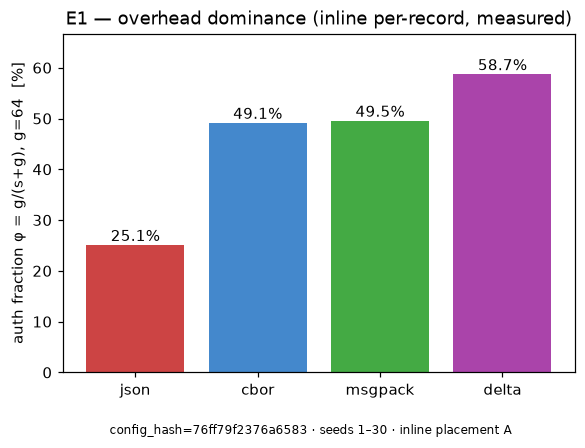
\includegraphics[width=0.7\textwidth]{fig_e1_dominance.png}
\caption{Authentication fraction across encodings. Every byte saved on the payload raises the
fraction spent on cryptography.}
\label{fig:e1}
\end{figure}

\begin{remark}[$s$ is not a property of the encoding alone]
The sizes above are measured over the first $\sim$50 seconds of each simulated flight. Sequence
numbers and timestamps grow with the record index, and variable-length encodings charge for the
extra digits, so JSON, CBOR and MessagePack all grow by 2--4\,B over a ten-times-longer window
while delta-CBOR stays flat --- it encodes differences. The bootstrap interval quoted for CBOR is
$\pm0.02$\,B and describes \emph{seed} variation; the systematic dependence on window length is
$\approx 2.7$\,B, roughly $150\times$ wider. The direction is conservative: a longer flight inflates
the baseline and leaves the optimum alone, so the reported saving is the pessimistic end.
\end{remark}

\section{E2 --- batching is the cure, and which ceiling binds}

Sweeping placement A against B across encodings and MTU budgets confirms \Cref{prop:t2}
qualitatively and \Cref{thm:t2a} quantitatively. At $M = 256$ the MTU binds and amplification is
operative; at $M = 576$ and $M = 1500$ freshness binds and the marginal value of compression is
$1.0000$ to twelve decimal places.

\textbf{The practical consequence.} On 802.11 the amplification law that motivates aggressive
compression is never operative. Compression still pays --- it pays exactly $1\times$.

\begin{figure}[h]
\centering

\includegraphics[width=0.7\textwidth]{fig_e2_batching.png}
\caption{Per-record cost against batch size. The curve flattens where the freshness ceiling takes
over from the frame-size ceiling.}
\label{fig:e2}
\end{figure}

\section{E3 --- the loss frontier}

Measured verifiability against batch size and loss probability, placement B versus D. Frame-level
batching Pareto-dominates block-level for all $V > (1-p)^2$, and at $\varepsilon = p$ block-level is
infeasible beyond one frame, as \Cref{thm:t3} requires.

\begin{remark}[What this experiment does and does not validate]
The emulator implements independent per-frame loss, which is also what the closed form assumes.
Agreement is therefore a \emph{consistency check}, not a validation of the loss model. What rescues
the ordering is \Cref{thm:t3c}, which holds for any stationary loss process, plus Gilbert--Elliott
simulation at matched mean rate showing $V_D$ approaching but never reaching $1-p$.
\end{remark}

\begin{figure}[h]
\centering

\includegraphics[width=0.7\textwidth]{fig_e3_frontier.png}
\caption{The loss-robustness frontier. Block-level authentication trades verifiability for bytes at
a rate the constraint does not permit.}
\label{fig:e3}
\end{figure}

\chapter{Results II --- Co-design and the Capacity Envelope}\label{ch:codesign}

\needswork{STATUS: DRAFTED. The ablation section deliberately narrows the thesis's own claim.}

\section{E5 --- the end-to-end configuration}

Exhaustive search over the full grid returns delta-CBOR, Ed25519, placement B, $b = 4$: $72.0$\,B
per record against $174.3$\,B for the compression-only baseline and $299.1$\,B for the naive one ---
a \textbf{$58.7\%$ total-byte reduction}.

\begin{remark}[Report the decomposition, never the bare authentication ratio]
The authentication-byte cut is $75.0\%$, and it is tempting to lead with it. It must not be led with,
because it reduces algebraically to $1 - 1/b$: invariant to the header, the signature size, the
encoding and the scheme. It is the definition of batching, not a result. The honest headline is the
\emph{total} byte reduction reported as a decomposition --- placement$\times$batching $79.2\%$,
encoding $20.8\%$, scheme byte-neutral.
\end{remark}

\begin{figure}[h]
\centering

\includegraphics[width=0.7\textwidth]{fig_e5_codesign.png}
\caption{End-to-end per-record cost against the two baselines.}
\label{fig:e5}
\end{figure}

\section{The factorial ablation, which narrows the claim}

A full factorial ablation over the four axes asks whether ``co-design'' is doing work that
single-axis optimisation would not.

\begin{itemize}
\item \textbf{Placement and batching couple exactly}, by $\ga(1 - 1/b)$ --- hence \emph{exactly
      zero} at $b = 1$, where placements A and B are byte-identical on a single-record frame.
\item \textbf{Encoding is perfectly separable.} Every interaction term is exactly zero, because $s$
      enters additively and therefore \emph{cannot} interact.
\item \textbf{The scheme axis is byte-degenerate} in this regime: the two $64$\,B schemes differ
      only in CPU cost.
\end{itemize}

An earlier claim that a smaller payload increases the value of batching was a \textbf{ratio-scale
artifact}: the absolute saving is $81.0$\,B for every encoding. The four-axis co-design claim was
overstated and is now precise. \textbf{No number moved --- only its interpretation.}

\begin{remark}
Note that $1 - 1/b$ is the same term as the warning above. The genuine coupling and the flattering
headline are the same algebra, seen from two directions.
\end{remark}

\section{E4 --- scheme selection on real hardware}

On ARM --- the deployment platform --- Ed25519 verification is $33.2\times$ cheaper than a BLS
pairing, which keeps Ed25519 optimal for self-batching at any plausible radio/CPU power ratio. The
ordering between Ed25519 and ECDSA-P256 \emph{flips} between x86 and ARM, so the choice is
platform-specific; the authentication-byte result is identical either way, since both are $64$\,B.

\begin{figure}[h]
\centering
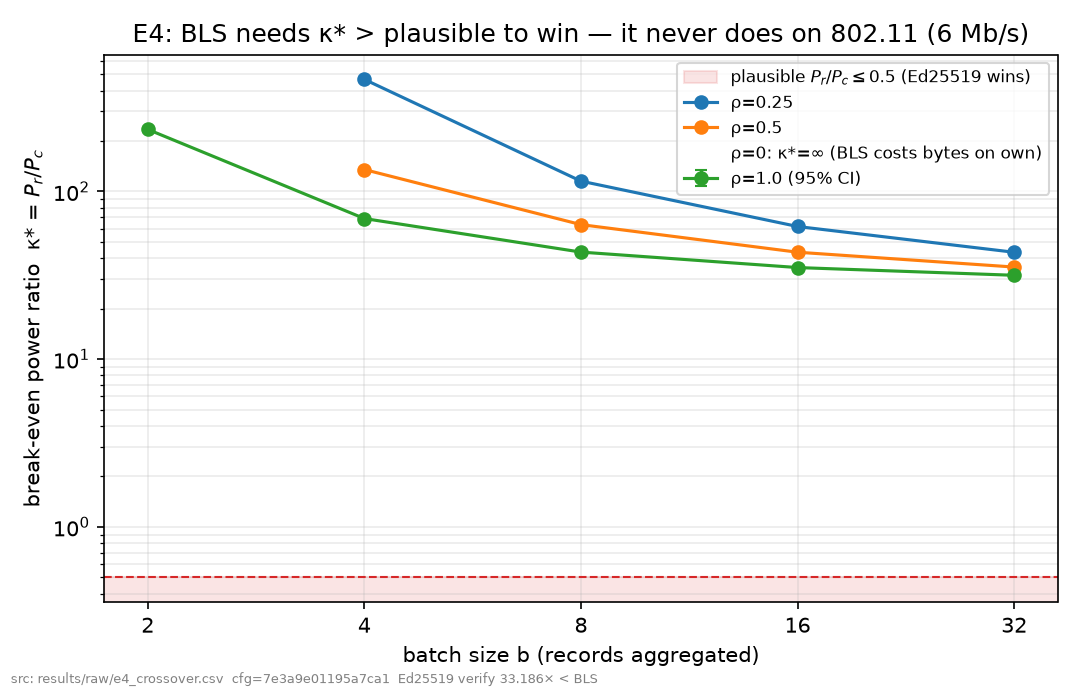
\includegraphics[width=0.7\textwidth]{e4_crossover.png}
\caption{The scheme crossover. BLS becomes worthwhile only in the cross-signer regime.}
\label{fig:e4}
\end{figure}

\section{E8 --- the capacity envelope}

Joining the byte model to the validated broadcast channel model turns ``how many bytes?'' into the
question an operator actually asks: \emph{how many UAVs, at what telemetry rate?}

\begin{table}[h]
\centering
\caption{Largest sustainable neighbourhood, reported at two thresholds because they answer
different questions. The per-run column is the reliability reading of the same criterion.}
\label{tab:envelope}
\begin{tabular}{lrrrrrr}
\toprule
configuration & $\Lambda_i$ & $\Dmax$ & $b$ & $\Nmax$ ($U{<}1$) & $\Nmax$ ($V$ mean) & ($V$ per run) \\
\midrule
\multicolumn{7}{l}{\emph{Primary: compliant with 3GPP TS 22.125}}\\
\textbf{optimized} delta/B & 50 & 100\,ms & 4 & \textbf{35} & \textbf{100} & 64--91 \\
A+CBOR (compression-only)  & 50 & 100\,ms & 1 & 18 & 31 & 24--29 \\
\midrule
\multicolumn{7}{l}{\emph{Relaxed freshness: same bytes, larger swarm, exceeds the standard}}\\
optimized delta/B & 20 & 250\,ms & 4 & 103 & 213 & 163--201 \\
A+CBOR            & 20 & 250\,ms & 1 & 32  & 88  & 54--80 \\
\bottomrule
\end{tabular}
\end{table}

The four ratios are $1.94\times$, $3.23\times$, $3.22\times$ and $2.42\times$.

\begin{remark}[Do not round this to ``about three times'']
The spread is $1.9$--$3.2\times$ and must be quoted as a range. An earlier draft of this work said
``$\approx 3\times$ holds across readings'', which is both false and precisely the kind of claim the
rest of this thesis exists to avoid. The co-design advantage is \emph{insensitive to the choice of
threshold} --- that is the defensible statement --- but it is not a single number.
\end{remark}

\begin{figure}[h]
\centering

\includegraphics[width=0.75\textwidth]{fig_envelope.png}
\caption{The feasibility envelope. The compression-only baseline runs out of channel where the
co-designed configuration does not.}
\label{fig:envelope}
\end{figure}

\section{What the envelope rests on}

The absolute capacities depend on a utilisation ceiling measured at one operating point and applied
across the envelope. \Cref{ch:validation} reports the experiment that tested that assumption, and
what it still leaves untested. The \emph{ratios} are protected by construction, because numerator
and denominator use the same ceiling; the absolute figures are not, which is why both are given.

\chapter{Model Validation and Hardware}\label{ch:validation}

\needswork{STATUS: DRAFTED.}

\section{Three independent implementations of the same physics}

The broadcast channel model is the load-bearing input to the capacity envelope, so it is validated
against two independent sources rather than one.

\begin{table}[h]
\centering
\caption{Saturation throughput (Mb/s), $1400$\,B broadcast frames. The slot-exact simulator was
written \emph{before} the published model was located and shares none of its assumptions.}
\label{tab:validation}
\begin{tabular}{rrrrrr}
\toprule
$N$ & published model & slot-exact sim & $\Delta$ & NS-3 & $\Delta$ \\
\midrule
5  & 4.3329 & 4.3305 & $-0.06\%$ & 4.3318 & $-0.03\%$ \\
10 & 3.1319 & 3.1321 & $+0.00\%$ & 3.1288 & $-0.10\%$ \\
20 & 1.7823 & 1.7830 & $+0.04\%$ & 1.7866 & $+0.24\%$ \\
35 & 1.2407 & 1.2407 & $-0.00\%$ & 1.2343 & $-0.51\%$ \\
50 & 1.2595 & 1.2585 & $-0.08\%$ & 1.2541 & $-0.43\%$ \\
\bottomrule
\end{tabular}
\end{table}

Agreement is $\leq 0.08\%$ against the independent simulator and $\leq 0.51\%$ against NS-3. Unicast
agrees with the acknowledged DCF model to $-0.40$/$+1.29\%$ across $N = 5$--$50$, with fixed-point
residuals below $10^{-12}$.

\begin{figure}[h]
\centering

\includegraphics[width=0.75\textwidth]{fig_ns3_bianchi.png}
\caption{Analytic models against simulation, both modes.}
\label{fig:validation}
\end{figure}

\section{The mechanism, confirmed by removing it}

The reason broadcast needs its own model is a specific asymmetry. A station that has just
transmitted redraws its backoff and may draw zero, taking the medium immediately after the
interframe space, while every station that deferred necessarily holds a counter of at least one. In
unicast the acknowledgement timeout blocks colliders from doing this; in broadcast nothing does.

The slot-exact simulator can disable \emph{exactly} that asymmetry and nothing else. Doing so
collapses it onto the naive reduction --- a $16.9\times$ gap at $N = 50$. \textbf{The mechanism
attribution is therefore not an inference from agreement; it is a controlled intervention.}

\begin{remark}[An expensive lesson]
This project used the naive reduction --- the unicast model with the acknowledgement removed and
the transmission probability fixed --- for several phases. It under-predicts by $16\times$ at
$N = 50$. The published broadcast model's own authors open by warning that unicast models cannot
simply be reduced for broadcast analysis. \emph{The failure was reading a model without reading its
preamble.}
\end{remark}

\section{A non-monotonicity that is real}

Saturation throughput is \textbf{not monotone decreasing} in $N$: it dips near $N \approx 35$ and
recovers. All three implementations reproduce it, so it is a property of the freeze-process series
rather than a bug --- each freeze stage contributes a hump peaking at a station count set by the
contention window.

This matters operationally. The capacity search breaks on the first violating $N$, which is valid
only if utilisation is monotone. It is --- because the explicit factor $N$ in the numerator outruns
the recovery --- but \textbf{that is an arithmetic accident, not a structural guarantee}, and it is
now verified exhaustively rather than assumed.

\section{Hardware}

Two Raspberry Pi 4 units in ad-hoc mode at $5$\,GHz measured broadcast link loss at
$p = 2.3 \times 10^{-4}$ and airtime at $1.995$\,ms per frame against $1.99$\,ms predicted --- an
independent check on the timing constants underlying every airtime figure in this thesis.

\begin{remark}[Two warnings, both earned]
This validates \emph{airtime}, not contention: one transmitter means zero contention, so the
broadcast contention model remains simulation-only.

And an initial $2.4$\,GHz sweep produced a tidy $97.45\%$ delivery figure that was \textbf{saturation
at the 802.11b $1$\,Mb/s broadcast basic rate}, not channel loss. It was caught by a pre-stated
prediction plus a load sweep, and is kept in the record labelled as what it was. Repeatability did
not protect against it --- the standard deviation across windows was small. \emph{A precisely
reproducible measurement of the wrong thing looks exactly like a good measurement.}
\end{remark}

\section{The utilisation ceiling, and a flaw in the author's own pre-registration}

The capacity envelope applies one measured utilisation ceiling to configurations whose frames span
$153$--$299$\,B, but that ceiling had only ever been measured at $288$\,B. A second sweep at
$174$\,B --- the compression-only baseline frame, which produces the denominators the capacity
ratios divide by --- tested it, with the prediction committed data-free beforehand.

\begin{center}
\begin{tabular}{lrr}
\toprule
& $288$\,B & $174$\,B \\
\midrule
$V \geq 0.95$ crossing & 2.435 & 2.367 \\
combined standard error & \multicolumn{2}{c}{$\pm 0.151$} \\
significance of the shift & \multicolumn{2}{c}{$0.45\sigma$} \\
\bottomrule
\end{tabular}
\end{center}

\textbf{Statistically indistinguishable across a $1.66\times$ change in frame size.} The universal
ceiling is justified and no published number moves.

\begin{remark}[The prediction that should not have been made]
The pre-registration also predicted a \emph{direction} --- that the crossing would drift higher ---
and offered a mechanism. It drifted lower, at $0.45\sigma$. The experiment has no power to resolve
the sign, so had the noise fallen the other way the author would have recorded a confirmation he
had not earned, and the mechanism offered is neither supported nor refuted.

This is recorded rather than quietly dropped because it is the same defect class the rest of this
thesis catalogues: \textbf{a number that looks like evidence and is not}. A directional prediction
needs a power estimate, or must be stated as a band. The load-bearing prediction did carry one,
which is why the run answers its question at all.
\end{remark}

\textbf{Still untested:} invariance in $N$. Both arms are at $N = 50$ while the envelope applies the
ceiling from $N = 2$ to $N = 213$. Frame-size invariance was the cheaper half of the assumption and
the half that varies across the envelope's rows; the other half is stated, not measured.

\chapter{The Low-Rate Regime and the Exclusion Bound}\label{ch:lowrate}

\needswork{STATUS: DRAFTED. This chapter carries the thesis's most durable result and also its
most uncomfortable self-correction. Both are stated here rather than in a limitations section.}

\section{Why the low-rate arm is a different regime, not a slower one}

The 802.11 numbers do not transfer. They differ by two to three orders of magnitude, and the
binding constraint differs \emph{in kind}: a regulatory airtime quota rather than a frame size or a
latency budget. This is the third regime in the taxonomy of \Cref{thm:t2a}:

\begin{center}
\begin{tabular}{lll}
\toprule
regime & what caps the batch & where \\
\midrule
MTU-limited & frame size & --- \\
freshness-limited & $\Lambda_i \Dmax$ & \textbf{802.11} \\
\textbf{duty-cycle-limited} & regulatory airtime quota & \textbf{low-rate} \\
\bottomrule
\end{tabular}
\end{center}

On this arm the arrival rate and the freshness are \emph{derived}, not configured: a frame of
airtime $T$ may repeat only every $T/\text{duty}$, so the sustainable rate and the staleness of the
oldest record are the same interval. There is no independent deadline to trade against bytes.

\section{The exclusion, and what part of it is arithmetic}

Applying \Cref{thm:t6} to EU868, with $\Hf = 44$\,B measured, $\ga = 64$\,B and $\smin = 13$\,B:

\begin{table}[h]
\centering
\caption{The EU868 partition. \textbf{Read the tier column, not just the verdict}: it says what
would have to change.}
\label{tab:t6}
\begin{tabular}{llrll}
\toprule
DR & payload $M$ & $\smax$ & tier & durability \\
\midrule
0, 1, 2 & 51\,B  & $-57$ & \textbf{signature} & \textbf{unconditional} \\
3       & 115\,B & $7$   & encoding & contingent --- see below \\
4, 5, 6 & 242\,B & $134$ & ---      & feasible \\
\bottomrule
\end{tabular}
\end{table}

\begin{figure}[h]
\centering
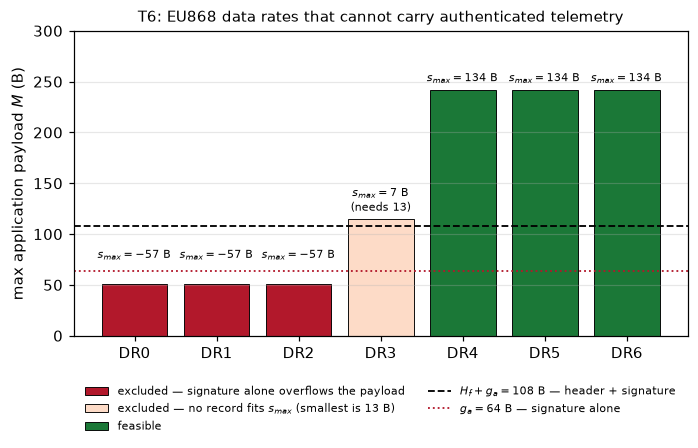
\includegraphics[width=0.75\textwidth]{fig_t6_exclusion.png}
\caption{Exclusion tiers across EU868 data rates.}
\label{fig:t6}
\end{figure}

\subsection{The three rates that cannot be rescued}

DR0--DR2 stay excluded \emph{with a zero-byte header and a one-byte record}. It is the signature
alone that does not fit: $64 > 51$. No header design, no encoding, no batching and no chain
placement reaches them. The only escape is a smaller authentication object, and the smallest
standardised one at comparable security is a $48$\,B compressed BLS12-381 G1 point --- which does
fit $51$\,B, and leaves \emph{three bytes} for the header and the record together.

\textbf{This is arithmetic. It does not move as hardware, models or schemes improve.} It is the
thesis's most durable claim and the reason the work is framed as a boundary.

\subsection{The fourth rate, which this thesis excluded by its own framing}

DR3 misses by six bytes. That margin rests on three constants, and \textbf{each of them is ours}:

\begin{enumerate}
\item $\Hf = 44$\,B, which is the \emph{top} of a measured $38$--$44$\,B range
      (\Cref{tab:hf}), and larger headers make exclusion more likely.
\item The payload column: published EU868 tables differ, and one source lists DR3 at $123$\,B where
      this work uses $115$\,B. At $123$\,B the residual is $15$\,B and \textbf{DR3 is feasible}.
\item $\smin = 13$\,B, the smallest record \emph{this design} can emit.
\end{enumerate}

\begin{remark}[The self-correction, stated plainly]
The frame header is $29$\,B of CBOR \emph{text key names}. The same seven keys encoded as small
integers cost $7$\,B --- the convention COSE and SenML already use. That single change takes
$\Hf$ from $44$ to $22$\,B, DR3's budget from $7$\,B to $29$\,B, and \textbf{makes DR3 feasible}.

The system-model chapter had always recorded that the header was untuned. The theory chapter had
always recorded that the bound depends on the header. \emph{Nobody put the two facts side by side.}
When they were, the headline moved from \textbf{four} excluded data rates to \textbf{three}.

Not even the record-field elision is required; halving the header suffices.
\end{remark}

\subsection{Why the smaller result is the better one}

Reporting three rather than four costs a memorable number and buys three things.

It is \emph{honest}: the four-rate claim was one reviewer's wire-format question away from being
wrong, and that reviewer would have been right. It is \emph{durable}: what remains cannot be
attacked by any framing work. And it makes the boundary \textbf{constructive} --- it says not only
where authentication cannot fit, but exactly what would have to change, and shows that for DR3 the
answer is a header redesign rather than new cryptography.

The tier taxonomy of \Cref{thm:t6} always named ``encoding'' as the tier compression can attack.
This is that tier being attacked, and moving, exactly as the taxonomy predicted.

\section{Per-frame chaining, and why the arms differ}

Moving the chain hash from per-record to per-frame is worth far more here than on 802.11, because
the regional payload limit binds --- so smaller records convert into \emph{more records per frame},
which the duty cycle turns directly into sustainable rate. Measured across DR4--DR6 it gives
$\approx 3.0\times$ the sustainable telemetry rate for the same regulatory budget.

\begin{figure}[h]
\centering

\includegraphics[width=0.7\textwidth]{fig_lora_chain.png}
\caption{Per-frame versus per-record chaining across data rates.}
\label{fig:lorachain}
\end{figure}

The 802.11 arm keeps per-record chaining, because freshness binds there and the same change buys
almost nothing in extra records --- too little to pay for losing independently-transmitted
per-record tamper evidence. \textbf{The two arms carry the same ledger in two framings, and that
asymmetry is the point rather than an inconsistency.}

\section{Capacity, and a threshold applied to the wrong thing}

Everything else in this arm is analytical and deliberately so --- time on air is a specification
formula and the sustainable rate is the duty cycle, both deterministic, so simulating them would be
circular. Exactly one quantity resists that: \emph{how many nodes can share the channel}, because
uplinks are pure ALOHA with no carrier sense.

Simulation at DR5 gives $\Nmax = 3$ against the $V \geq 0.95$ criterion.

\begin{remark}[Never quote this bare]
The bootstrap interval is $[2, 3]$ --- a knife edge --- and at the certified $N = 3$, \textbf{nine of
thirty seeds fail the very criterion being certified}. Under a per-realisation reading, where at
least $95\%$ of runs must individually meet $V$, the answer is \textbf{1}, not 3.

Both are computed and emitted. The decision to headline the mean is recorded as a decision, and it
was safe to take only because the comparative result survives either reading.
\end{remark}

An earlier value of $\Nmax = 5$ came from a three-seed sample against a bimodal distribution and is
retracted; the artifact that produced it is retained, renamed and superseded.

\subsection{External corroboration, quoted as a curve}

An external hardware-grounded model gives $\Nmax = 4$ where this work gives $3$.

\begin{remark}[Two cautions about that comparison]
Their $\Nmax$ is decided at $N = 4$ and $N = 5$, both inside the region their own fit is
intercept-dominated: the polynomial predicts $1.78\%$ loss at \emph{zero} transmitters, roughly
$40\%$ of the entire loss budget the criterion allows. Forcing the fit through the origin would give
them $\Nmax = 5$, \emph{widening} the gap --- so quoting $4$ is the conservative choice.

And the pessimism ratio is not a single number. It runs $0.91\times$ at $N = 2$, where \emph{this
work is the more optimistic model}, through $1.07\times$ at $N = 3$, to $2.1\times$ from $N = 10$
upward. The sign changes in exactly the region where $\Nmax$ is decided. An earlier finding in this
project quoted a single ratio in the wrong direction and had to be retracted.
\end{remark}

\section{Scope of this chapter}

This is simulation and analysis, not measurement. No radio was metered, and there is no energy
column --- the only measured radio power in this project is a Wi-Fi figure, and reusing it for a
different transceiver would be fabrication. Airtime per record is reported instead: it is what the
regulator rations, and it is computed rather than assumed.

\chapter{Reproducibility, Defects and Research Integrity}\label{ch:reproducibility}

\needswork{STATUS: DRAFTED. This chapter is unusual for a thesis and deliberate. It reports the
errors found in this project's own results. Examiners should read it as the methodological
contribution it is intended to be, not as an admission appended to a limitations section.}

\section{Why this chapter exists}

Most theses report what was found. This one also reports \emph{what was found to be wrong, and how}.
The justification is not confession but transferability: the defects catalogued below are not
peculiar to this work, and several of them survived safeguards that are widely considered
sufficient --- version control, a green test suite, seeded runs, committed raw data.

Ten results in this project moved after they were first recorded. Only four were catchable by
running more seeds. Two were \emph{protected by passing tests}. Three were contradictions between a
paper and the artifact that generated it.

\section{The defect taxonomy}

\begin{center}
\begin{tabular}{p{2.2cm}p{5.6cm}p{5.2cm}}
\toprule
class & mechanism & instance in this work \\
\midrule
\textbf{C1} & small-sample mean lands the wrong side of a threshold & four headline numbers; a
capacity value $5 \rightarrow 3$ \\
\textbf{C2} & an unverified constant on the measurement path & the $2.4$\,GHz basic-rate
saturation; the frame header treated as a constant \\
\textbf{C3} & a threshold applied to a mean rather than a distribution & the capacity criterion;
the utilisation crossing \\
\textbf{C4} & a configuration change that perturbs the random realisation & simulator stream
displacement under mobility \\
\textbf{C5} & a claim wider than the experiment supports & two-node hardware described as
validating contention \\
\bottomrule
\end{tabular}
\end{center}

\begin{remark}[The load-bearing observation]
\textbf{More seeds fixes only C1.} C2--C5 are immune to sample size. ``We ran thirty seeds'' is
therefore not a statement of correctness, and the discipline installed after the C1 failures gave
no protection at all against the C2 failures found later.
\end{remark}

\section{An automated staleness gate, and what it does not cover}

Every model-derived artifact is re-derived from current code on every run and compared row by row;
a single differing value fails the build. This makes silent staleness of \emph{derived} data
impossible.

It does not make staleness impossible. Two limits were found the hard way:

\begin{itemize}
\item \textbf{Scope.} Every drift guard originally parsed the paper. The specification documents
were outside that scope, so corrections propagated into the paper and not into the documents for
three weeks --- including a table built verbatim on data the project had already purged and
superseded.
\item \textbf{Direction.} Retracting a finding in a register does not remove it from the prose. One
retracted claim was found alive in the paper months later, one hundred lines below a sentence
stating the opposite, and later again in the open-items register. \textbf{When you retract, grep the
whole repository.}
\end{itemize}

\section{Practices that earned their place}

\begin{description}
\item[Pre-registration, committed data-free.] Predictions are committed as their own commit before
data exist, so the ordering is third-party checkable. This cost the project a claim once: an
assertion of pre-registration was \emph{withdrawn} rather than reconstructed, because writing an
expectations file after results are known manufactures evidence.

\item[Stating the expected value before measuring.] This is what caught the $2.4$\,GHz
basic-rate artifact, which repeatability would never have caught.

\item[Retaining a discarded model as a labelled failure curve.] The naive broadcast reduction
remains in the codebase, clearly marked, so the $16\times$ error it produces can be shown rather
than described.

\item[Keeping per-seed raw data, not summaries.] This allowed validation bands to be re-derived at
thirty seeds without re-simulating.

\item[An independent second implementation.] The slot-exact simulator, written before the published
model was found, shares none of its assumptions and is what turns agreement into evidence.
\end{description}

\section{Two defects worth stating individually}

\subsection{A test that asserted a bug}

A utilisation function returned exactly zero for a single node, with a unit test asserting that a
lone sender never contends. The function conflated \emph{contention} with \emph{utilisation}: a lone
sender does not collide but still occupies airtime, and returning zero declared a single node able
to carry unbounded traffic. The defect was harmless until another result began reporting
single-node cases --- \textbf{and it was protected by a passing test that had encoded the wrong
behaviour as intended behaviour}.

\subsection{A criterion that could not fail}

The project pre-registered a success criterion requiring at least a $40\%$ reduction in
authentication bytes, and committed it to version control two days before the result existed. The
ordering is genuine and verifiable.

The quantity it tests, however, reduces exactly to $1 - 1/b$. The threshold is therefore
$b \geq 2$ --- independent of encoding, scheme, placement, header size and signature size. The
companion condition on verifiability is satisfied by construction with zero margin. \textbf{No
configuration that batches at all could have failed the test.}

The pre-registration is real and worth keeping; what had to go was the implication that it
constituted a risk the design might not have survived.

\section{What a reader should take from this}

Three times in this project a claim survived because two facts were each individually recorded and
never placed side by side. A register that stores facts separately does not compose them.
\textbf{Only re-derivation does.}

\needswork{TO ADD: a comparison with the reproducibility literature --- the simulation-credibility
lineage in particular --- so this chapter reads as a contribution to that conversation rather than
as a project post-mortem. The companion methods paper does this; the material needs porting.}

\chapter{Conclusions, Limitations and Future Work}\label{ch:conclusions}

\needswork{STATUS: DRAFTED. The future-work section is the one most likely to be examined for
evidence that the candidate understands the work's boundaries; it is written accordingly and
deliberately does not oversell.}

\section{What this thesis establishes}

\begin{enumerate}
\item After compression, authentication --- not data --- is the dominant on-air cost of a
tamper-evident UAV telemetry ledger. At the smallest encoding studied, the signature is larger than
the record it signs.

\item Frame-level self-batching is the correct placement, and it Pareto-dominates block-level
aggregation under \emph{any} stationary loss process, not merely under the independent-loss
assumption the emulator implements.

\item On IEEE 802.11 the freshness deadline binds before the frame size does, so the amplification
law that motivates aggressive compression is never operative: compression pays exactly $1\times$.
On low-rate links the frame size binds and the leverage is real. \textbf{The regimes are different
in kind.}

\item Three of seven EU868 data rates admit no per-frame-verifiable telemetry at any encoding,
batch, header or chain design, because a $64$\,B signature does not fit a $51$\,B payload. This is
arithmetic and cannot move.

\item Joined to a validated channel model, the co-designed configuration sustains
$1.9$--$3.2\times$ the neighbourhood of an inline baseline, at $58.7\%$ fewer on-air bytes, at an
operating point compliant with 3GPP TS~22.125.

\item Of the four design axes, only placement and batching genuinely interact. The four-axis
co-design claim, as originally stated, was overstated.
\end{enumerate}

\section{Limitations, stated as such}

\subsection{Modelling scope}

The single collision domain admits no spatial reuse and no hidden terminals; a real formation has
both, one helping and one hurting. Mobility was tested and found null for collision-limited
capacity, but per-frame Doppler is unmodelled --- the null result means mobility does not change
\emph{collision-limited capacity}, not that mobility is harmless to a link. Loss is independent per
frame; the ordering result survives correlation but absolute verifiability figures do not. The
keyframe interval is fixed and unoptimised. Post-quantum sizes are projections, not
implementations.

\subsection{Validation scope}

Simulation validates \emph{throughput}. Latency, energy and loss behaviour are not validated by it,
and ``simulation-validated'' must not be read as more. Hardware validates \emph{airtime} on a
two-node link; contention remains simulation-only. The utilisation ceiling is measured at one node
count. Composed energy is a lower bound by roughly $10$--$14\%$, and the residual is uncharged
prototype framing overhead --- measured, stated, not corrected away.

\subsection{The low-rate arm}

Analysis and simulation only: no radio metered, no energy column, one spreading factor per run.
The capacity figure is a within-one-spreading-factor bound, not a network capacity, and its
confidence interval is a knife edge.

\subsection{The boundary itself}

Three of the four excluded data rates are arithmetic. The fourth was excluded by this design's own
frame header, and this thesis says so and quantifies the recovery. A reader should treat the
three-rate claim as durable and the fourth as an engineering statement about \emph{this} wire
format.

\section{Future work}

\subsection{Immediately available, and cheap}

\begin{description}
\item[Invariance of the utilisation ceiling in $N$.] Frame-size invariance was measured; node-count
invariance was not. One additional sweep closes it, and the scenario already exists.

\item[Pricing implicit certificates.] The certificate accounting charges an explicit certificate
periodically. Implicit (ECQV) certificates are the standard smaller alternative and were never
modelled. The current charge is an upper bound, which cuts against this work's own comparison ---
so the gap is safe but should be closed.

\item[An integer-keyed wire profile, adopted rather than measured.] \Cref{ch:lowrate} measures it
and declines to adopt it, because the format is frozen for reproducibility. A successor should
adopt it, re-freeze, and report the boundary that results --- which will be a \emph{smaller}
exclusion and a better-engineered system.
\end{description}

\subsection{Substantial, and worth doing}

\begin{description}
\item[Channel-access delay in the freshness model.] The freshness constraint that \emph{sets} the
batch omits the dominant delay term at high load. It is currently mitigated by reporting
utilisation alongside, not by fixing the model. A DCF access-delay term would make the freshness
constraint credible at high utilisation, where it currently is not.

\item[Multi-spreading-factor capacity on the low-rate arm.] Each run fixes one data rate,
forfeiting the quasi-orthogonality that supplies much of a real deployment's capacity. That answers
a different question --- deployment capacity rather than per-configuration feasibility --- and it
is the question an operator would ask next.

\item[Contention on real hardware.] Two radios validate airtime; the contention model, which
carries the capacity envelope, remains simulation-only. A rig with enough nodes to reach the
interesting region of the curve is the single most valuable missing measurement in this thesis.

\item[A post-quantum arm that is implemented rather than projected.] The projections show that
batching cannot rescue post-quantum signature sizes, because freshness caps the batch and one
signature plus header already exceeds the frame budget. That is a strong negative result and it
deserves measurement rather than arithmetic.
\end{description}

\subsection{Speculative, and stated as such}

The exclusion bound is link-agnostic. Instantiating it on other constrained bands --- and on the
signature sizes the post-quantum standards actually mandate --- would say which of tomorrow's radio
and cryptographic combinations are feasible before either is deployed. That is the natural
generalisation, and it is the one this author would pursue.

\section{Closing}

This thesis introduces no new cryptographic primitive and makes no claim to one. Its contribution
is a reproducible co-design of existing, standardised components; the quantified trade-offs that
co-design entails; the boundary beyond which no choice of those components helps at all; and an
account --- unusually explicit for a thesis --- of the errors made in establishing that boundary and
the classes of defect that survived the safeguards intended to prevent them.

The most durable result here is also the smallest one that survived scrutiny: on the longest-range
EU868 data rates, a $64$-byte signature does not fit a $51$-byte payload, and nothing in the design
space changes that.


\bibliographystyle{IEEEtran}
\bibliography{refs}

\end{document}
